\documentclass[tikz,border=5mm]{standalone}
\usepackage[T1]{fontenc}
\usepackage{fontspec}
\setmainfont{Fira Sans}[
  BoldFont=Fira Sans Bold,
  ItalicFont=Fira Sans Italic,
]
\usetikzlibrary{positioning, arrows.meta, shadows.blur, calc, patterns}

\definecolor{mTeal}{HTML}{2B7A78}
\definecolor{mBrown}{HTML}{C9956B}
\definecolor{mGray}{HTML}{888888}
\definecolor{mBg}{HTML}{FAFAFA}

\begin{document}
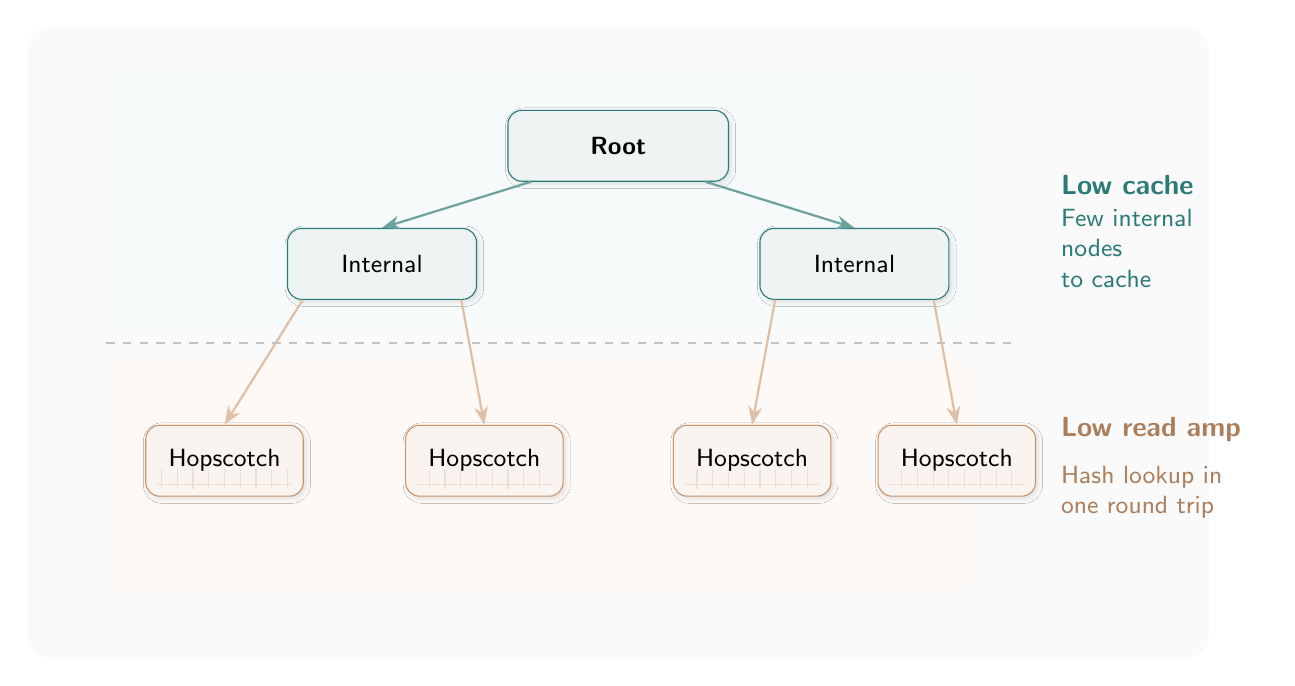
\begin{tikzpicture}[
  every node/.style={font=\sffamily},
  inode/.style={draw=mTeal, fill=mTeal!8, rounded corners=5pt,
                minimum width=2.4cm, minimum height=0.9cm, font=\sffamily\small,
                blur shadow={shadow blur steps=6, shadow xshift=0.3mm,
                shadow yshift=-0.3mm, shadow opacity=12}},
  lnode/.style={draw=mBrown, fill=mBrown!10, rounded corners=5pt,
                minimum width=2cm, minimum height=0.9cm, font=\sffamily\small,
                blur shadow={shadow blur steps=6, shadow xshift=0.3mm,
                shadow yshift=-0.3mm, shadow opacity=12}},
  >=Stealth,
]
  % Background
  \fill[mBg, rounded corners=8pt] (-7.5,-3) rectangle (7.5,5);

  % Region labels
  \fill[mTeal!4, rounded corners=6pt] (-6.5,1.2) rectangle (4.5,4.5);
  \fill[mBrown!6, rounded corners=6pt] (-6.5,-2.2) rectangle (4.5,0.8);

  % Internal nodes
  \node[inode, minimum width=2.8cm, font=\sffamily\small\bfseries] (root) at (0,3.5) {Root};
  \node[inode] (i1) at (-3,2) {Internal};
  \node[inode] (i2) at (3,2) {Internal};

  % Leaf nodes with hash pattern hint
  \node[lnode] (l1) at (-5,-.5) {Hopscotch};
  \node[lnode] (l2) at (-1.7,-.5) {Hopscotch};
  \node[lnode] (l3) at (1.7,-.5) {Hopscotch};
  \node[lnode] (l4) at (4.3,-.5) {Hopscotch};

  % Small hash indicators inside leaves
  \foreach \n in {l1,l2,l3,l4} {
    \draw[mBrown!30, thin] ($(\n.south west)+(0.15,0.1)$) grid[step=0.2] ($(\n.south east)+(-0.15,0.35)$);
  }

  % Edges
  \draw[->, thick, mTeal!70] (root.south west) ++(0.3,0) -- (i1.north);
  \draw[->, thick, mTeal!70] (root.south east) ++(-0.3,0) -- (i2.north);
  \draw[->, thick, mBrown!60] (i1.south west) ++(0.2,0) -- (l1.north);
  \draw[->, thick, mBrown!60] (i1.south east) ++(-0.2,0) -- (l2.north);
  \draw[->, thick, mBrown!60] (i2.south west) ++(0.2,0) -- (l3.north);
  \draw[->, thick, mBrown!60] (i2.south east) ++(-0.2,0) -- (l4.north);

  % Dashed separator
  \draw[dashed, mGray!50, thick] (-6.5,1) -- (5,1);

  % Annotations
  \node[mTeal, font=\sffamily\bfseries, anchor=west] at (5.5,3) {Low cache};
  \node[mTeal, font=\sffamily\small, anchor=west, text width=2.5cm] at (5.5,2.2) {Few internal nodes\\to cache};

  \node[mBrown!85!black, font=\sffamily\bfseries, anchor=west] at (5.5,-.1) {Low read amp};
  \node[mBrown!85!black, font=\sffamily\small, anchor=west, text width=2.5cm] at (5.5,-.9) {Hash lookup in\\one round trip};
\end{tikzpicture}
\end{document}
